\section{Discusión}

%destacar rdtsc
Tratándose de implementaciones en lenguaje en ensamblador, uno de las cuestiones que más tuvimos en cuenta y analizamos fue, por supuesto, la eficiencia de los algoritmos. Como ya dijimos, lo que hicimos fue medir la cantidad de clocks de procesador que cada función (incluso la de OpenCV y la que escribimos en C) consumen. Esto se logró mediante invocaciones desde C a la función \texttt{rdtsc} de lenguaje ensamblador.

El resultado que obtuvimos en ese sentido fue, como esperábamos, que nuestras implementaciones en ensamblador no alcanzaron la rapidez de la implementación de OpenCV, y que la implementación hecha en C fue aún más lenta. Los siguientes gráficos reflejan estas diferencias para imágenes de distintos tamaños.\footnote{\emph{ Las ejecuciones fueron realizadas en una PC: MSI Wind U100 con procesador Intel Atom N270 - 1Gb de RAM y bajo el S.O. Ubuntu Netbook Remix 9.04}}

%%

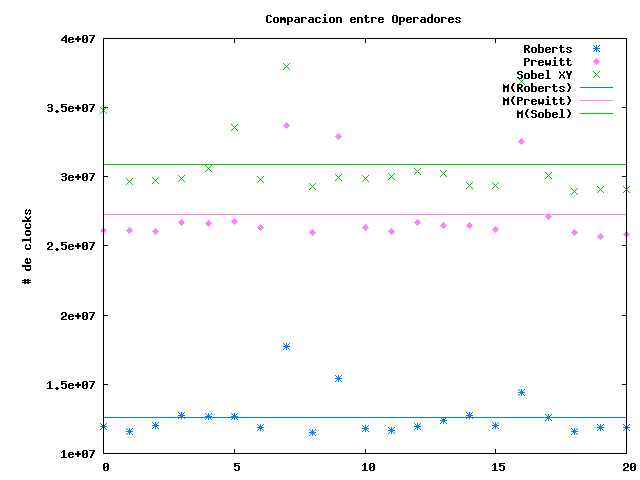
\includegraphics[scale=0.5]{graf1.png}

\medskip

\begin{center}
\begin{tabular}{lrrr}
\cr  & Roberts & Prewitt & Sobel\\
\hline
\emph {Media} & 12618185 & 27276745 & 30886607 \\
\emph {Desvío} & 1511854 & 2448652 & 2598392\\
\emph {Max} & 17743236 & 33694296 & 37954836\\
\emph {Min} & 11549460 & 25707576 & 28905552\\
\hline \\
\end{tabular}
\end{center}



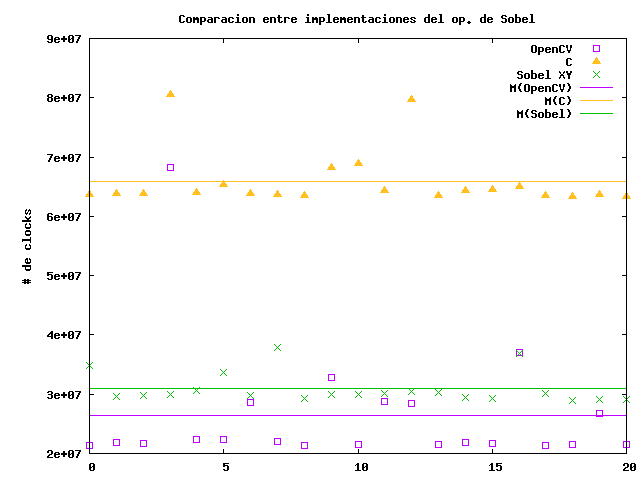
\includegraphics[scale=0.5]{sobels.png}

\medskip

\begin{center}
\begin{tabular}{lrrr}
\cr  & OpenCV & C & ASM \\
\hline
\emph {Media} & 26412756 & 65944312 & 30886607 \\
\emph {Desvío} & 10563470 & 4921205 & 2598392\\
\emph {Max} & 68276028 & 80518500 & 37954836\\
\emph {Min} & 21301152 & 63370956 & 28905552\\
\hline \\
\end{tabular}
\end{center}



%%

La diferencia de eficiencia entre la implementación en C y las hechas en ensamblador tiene un motivo claro y conocido. Por naturaleza, los lenguajes de programación de más alto nivel nos abstraen de muchas cuestiones de implementación, pero a la vez nos quitan control sobre esa implementación. Mientras en ensamblador usamos directamente los registros del procesador (memoria más rápida de la máquina) en C éstos se usan de manera interna y el programador trabaja con datos en memoria RAM.

Esta razón bastaría para justificar las diferencias de rendimiento, pero no es la única: además, el sólo hecho de estar programando en un lenguaje de nivel superior hace que el programador ponga menos atención en los detalles de eficiencia y más en otros aspectos como la legibilidad del código o su reutilizabilidad.

En cambio, el motivo de la diferencia de rendimiento entre nuestras implementaciones en ensamblador y la de OpenCV resulta menos evidente. De hecho no estudiamos el código que utiliza OpenCV. Sabemos, sin embargo, que nuestras implementaciones no aprovechan al máximo las posibilidades de los procesadores, a diferencia de las de OpenCV que seguramente utilizan capacidades más avanzadas y/o específicas de los mismos como por ejemplo el uso de MMX, SSE, etc..

Un ejemplo que se nos ocurre es la saturación: nosotros, para cada píxel, verificamos si el resultado está por debajo de 0 o por encima de 255 para ajustarlo. Estos chequeos y ajustes consumen un tiempo significativo de ejecución; es claro que usando aritmética saturada nativa del procesador se mejoraría mucho la performance.

Otra característica que imaginamos se podría aprovechar es la paralelización: al tratarse de cálculos sencillos y repetitivos podrían venir bien las instrucciones de datos empaquetados.

También resulta interesante observar en qué medida se aceleró el algoritmo cuando eliminamos los accesos a memoria innecesarios que realizábamos al utilizar la pila en lugar de sólo los registros. El gráfico que sigue compara el rendimiento de la primera implementación en ensamblador que hicimos (que aplicaba Roberts en X usando la pila) con la definitiva (que minimiza los accesos a memoria y aplica Roberts en ambas direcciones). Es notorio que, aunque la primera implementación realiza menos cálculos pues aplica una sola matriz en lugar de dos, sea tanto menos eficiente por no aprovechar al máximo los registros del procesador.

%%

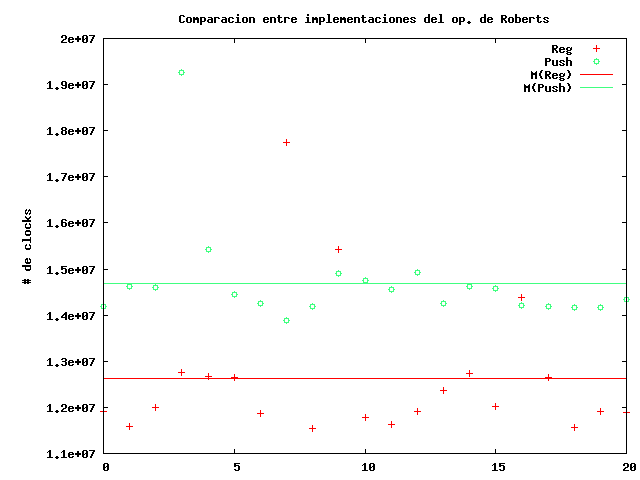
\includegraphics[scale=0.5]{roberts.png}

\medskip

\begin{center}
\begin{tabular}{lrr}
\cr  & ``Reg'' & ``Push''  \\
\hline
\emph {Media} & 12618185 & 14692721  \\
\emph {Desvío} & 1511854 & 1105330 \\
\emph {Max} & 68276028 & 19269852 \\
\emph {Min} & 11549460 & 13878600 \\
\hline \\
\end{tabular}
\end{center}

%%
